% This file defines the command for plotting the Sigmoid and Tanh functions.
% It can be compiled standalone or included in a larger document.

\ifdefined\ispartofbook
\else
  % --- Standalone Compilation Preamble ---
  \documentclass[tikz, border=10pt]{standalone}
  \usepackage{tikz}
  \usetikzlibrary{arrows.meta}
  \begin{document}
\fi

% --- THE DIAGRAM COMMAND ---
\newcommand{\saturatingplot}{%
    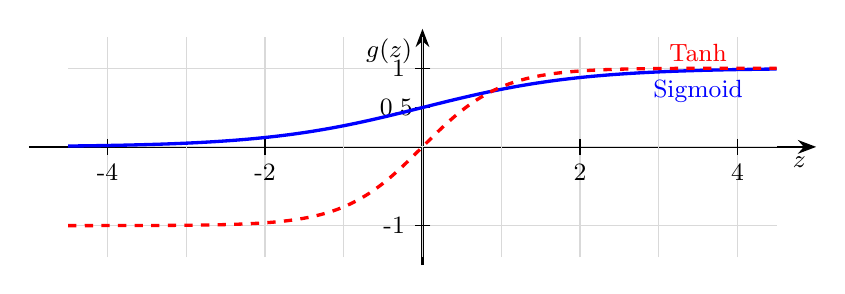
\begin{tikzpicture}[
        font=\sffamily,
        every node/.style={font=\small}
    ]
    % Axes
    \draw[-Stealth, thick] (-5,0) -- (5,0) node[below left] {$z$};
    \draw[-Stealth, thick] (0,-1.5) -- (0,1.5) node[below left] {$g(z)$};

    % Grid
    \draw[gray!30, thin, step=1] (-4.5,-1.4) grid (4.5,1.4);

    % Axis labels
    \foreach \x in {-4, -2, 2, 4}
        \draw (\x, 0.1) -- (\x, -0.1) node[below] {\x};
    \foreach \y in {-1, 1}
        \draw (0.1, \y) -- (-0.1, \y) node[left] {\y};
    \node[left] at (0, 0.5) {0.5};
    \draw (0.1, 0.5) -- (-0.1, 0.5);


    % Sigmoid function plot
    \draw[blue, very thick, smooth, domain=-4.5:4.5, samples=100] plot (\x, {1/(1+exp(-\x))});

    % Tanh function plot
    \draw[red, very thick, dashed, smooth, domain=-4.5:4.5, samples=100] plot (\x, {tanh(\x)});
    
    % Legend
    \node[blue] at (3.5, 0.7) {Sigmoid};
    \node[red] at (3.5, 1.2) {Tanh};
    
    \end{tikzpicture}%
}

\ifdefined\ispartofbook
  % This part is intentionally left blank when included in the main book.
  % The \newcommand is defined, and the chapter file is responsible for calling it.
\else
  % This part is for standalone compilation of the image.
  \saturatingplot
  \end{document}
\fi
